% Application - Prototypes
%%%%%%%%%%%%%%%%%%%%%%%%%%%%%%%%%%%%%%%%%%%%%

% FR
Avant d'entamer le développement de l'application, il est nécessaire de faire un état du besoin et des attentes. Ainsi, en structurant notre interface il sera plus facile de procéder à son développement graphique, d'anticiper les classes et fonctions nécessaires aux traitements. Dans un premier temps, nous allons structurer nos interfaces afin d'être au plus proche des attentes utilisateurs, puis nous détaillerons les outils à notre disposition et comment ils fonctionnent, et enfin nous procèderons au dévelopement de l'application cliente.

% EN
%Before starting the development of the application, it is necessary to make a statement of needs and expectations. Thus, by structuring our interface will make it easier to conduct its graphic development, anticipate the classes and functions necessary for treatment. Initially, we will structure our interfaces in order to be closer to the users expectations, then we will detail the tools available and how they work, and then we will proceed to the developement of the client application.

%%%%%%%%%%%%%%%%%%%%%%%%%%%%%%%%%%%%%%%%%%%%%%%%%%%%%%%%%%%%%%%%%%%%%%%%%
% FR
\section{Prototypes}

% EN
%\section{Prototypes}

% FR
Dans ce paragraphe nous allons détailler chacune des interfaces qui seront implémentées dans l'application. L'application sera construite sous deux angles différents :
\begin{description}
  \item[La partie cartographique :] \hfill \\ contenant une carte de base et dont les outils se superposent à cette dernière
  \item[La partie site web :] \hfill \\ contenant des outils indépendants de la carte
\end{description}

% EN
% In this section we will detail each of the interfaces that will be implemented in the application. The application will be built in two different ways:
% \begin{description}
%   \item[Map content :] \hfill \\ containing a basemap and whose tools are over the map
%   \item[Website content :] \hfill \\ containing independent map tools
% \end{description}

% FR
\subsection{Partie cartographique}

% EN
%\subsection{Map content}

% FR
Le contenu cartographique détermine la base de notre application. En effet, cette dernière est constituée de trois éléments important : le fond de carte, la table des matières et les boutons d'interraction avec la carte.

% EN
%The map content determines the basis of our application. Indeed, the latter consists of three major components: the base map, table of contents and the interraction with map buttons.



% BASEMAP
% ----------------------------------------------

\begin{figure}[ht]
  \centering
  \begin{subfigure}[b]{0.6\textwidth}
    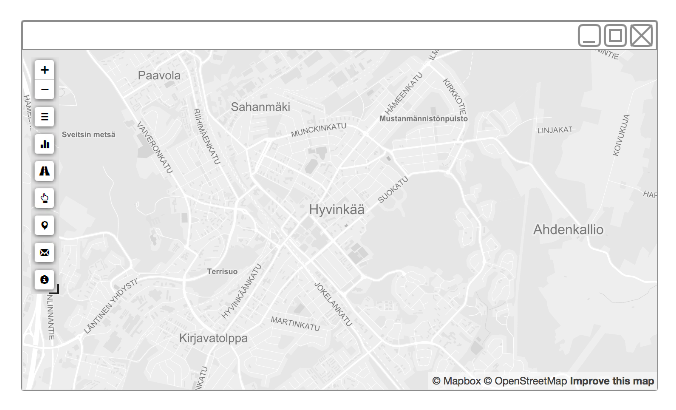
\includegraphics[width=\textwidth]
      {img/c02-application/png/web-basemap.png}
    \caption{Web}
  \end{subfigure}
  ~
  \begin{subfigure}[b]{0.2\textwidth}
    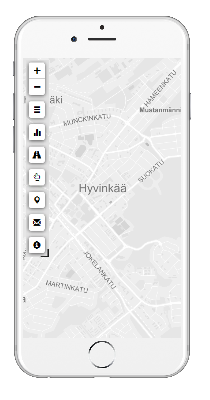
\includegraphics[width=\textwidth]
      {img/c02-application/png/mobile-basemap.png}
    \caption{Mobile}
  \end{subfigure}
  \caption{Application: Basemap}
\end{figure}

% EN
%The base map allows you to locate geographically in a recognizable environment. It shall be set up raster image on which we will be able to overlay vector data from the server. For our application we will build on the maps tiles proposed by MapBox.



% FR 
Le fond de carte permet de se repérer géographiquement dans un environnement reconnaissable. Il est consitué d'image raster sur lesquelles on va pouvoir superposer les données vectorielles issues du serveur. Pour notre application nous allons nous appuyer sur les fonds de carte proposé par MapBox.


% TOC
% ----------------------------------------------

\begin{figure}[ht]
  \centering
  \begin{subfigure}[b]{0.6\textwidth}
    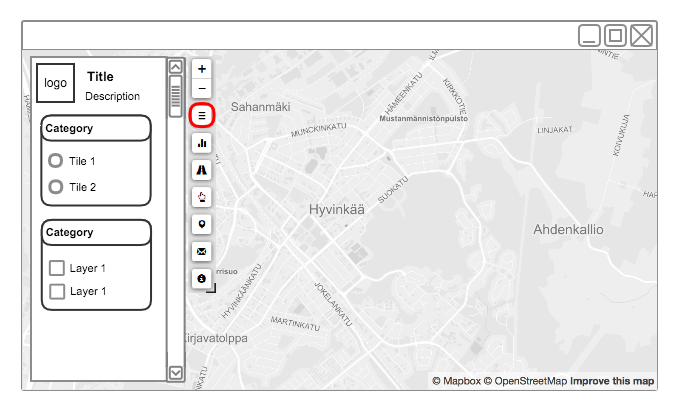
\includegraphics[width=\textwidth]
      {img/c02-application/png/web-basemap-toc.png}
    \caption{Web}
  \end{subfigure}
  ~
  \begin{subfigure}[b]{0.2\textwidth}
    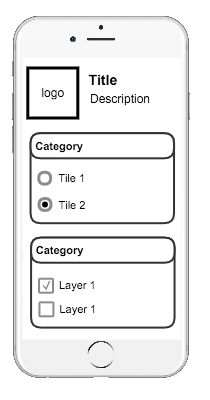
\includegraphics[width=\textwidth]
      {img/c02-application/png/mobile-basemap-toc.png}
    \caption{Mobile}
  \end{subfigure}
  \caption{Application: Table Of Content}
\end{figure}

% FR
La table des matières, ou \textit{Table of Content} (en anglais, abrégé TOC), permet de lister les élements de la carte et de pouvoir interagir avec eux. Elle contiendra les différentes couches, ou \textit{Layer} en anglais, constitutives de l'application. Des checkbox ou bouton radio devraient s'y trouver pour afficher ou masquer des éléments.

Les boutons d'interractions sont de trois types : le déclenchement d'action par dessus la carte (popup), le déclenchement d'action avec une interraction sur la carte, ou l'ouverture d'une page spécifique du minisite.

% EN
%The table of contents (abbreviated TOC) can list the elements of the map and interact with them. It will contain the different layers component of the application. The checkbox or radio button should be there to show or hide items.

%The interractions buttons are of three types: the onset of action over the map (popup), the onset of action with interraction on the map (marker), or open a specific page of the mini-website.

% SEARCH POINTER
% ----------------------------------------------

% FR
Parmis les boutons d'action sur la carte, un outils indispensable est la recherche d'itinéraire. Ce bouton permet d'activer la dépose de marker à la main directement sur la carte pour placer deux points qui serviront de départ et d'arrivée. Après avoir déposé les markers, un itinéraire le plus court est calculé et affiché sur la carte.

% EN
%Among the action buttons on the map, an indispensable tool is the route search. This button turns the marker removal by hand directly on the map to place two points that serve as departure and arrival. After dropping the markers, the shortest route is calculated and displayed on the map.

\begin{figure}[ht]
  \centering
  \begin{subfigure}[b]{0.6\textwidth}
    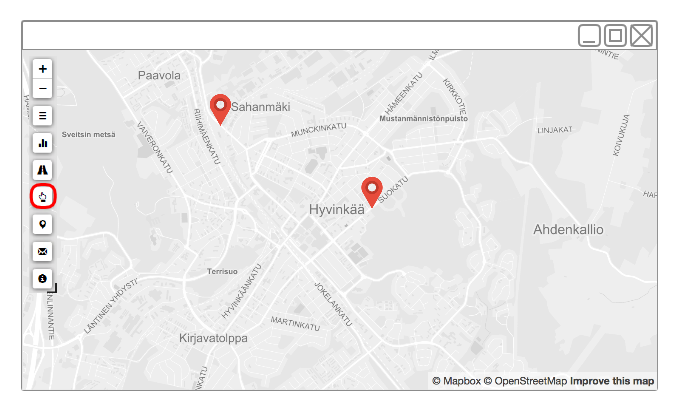
\includegraphics[width=\textwidth]
      {img/c02-application/png/web-basemap-search.png}
    \caption{Web}
  \end{subfigure}
  ~
  \begin{subfigure}[b]{0.2\textwidth}
    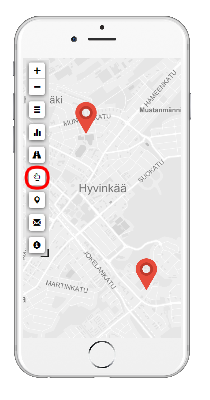
\includegraphics[width=\textwidth]
      {img/c02-application/png/mobile-basemap-search.png}
    \caption{Mobile}
  \end{subfigure}
  \caption{Application: SearchPointer}
\end{figure}

% FOCUS
% ----------------------------------------------

% FR
Un autre des outils nécessaires au bon fonctionnement de l'application est un bouton permettant de se géolocaliser. Ce bouton ouvre une popup par dessus la carte permettant de choisir de se localiser par mot clef ou bien par coordonnées (latitude et longitude).

% EN
%Another of the tools necessary for the application is a button to geotag. This button opens a popup over the map to choose to locate by keyword or by coordinates (latitude and longitude).

\begin{figure}[ht]
  \centering
  \begin{subfigure}[b]{0.6\textwidth}
    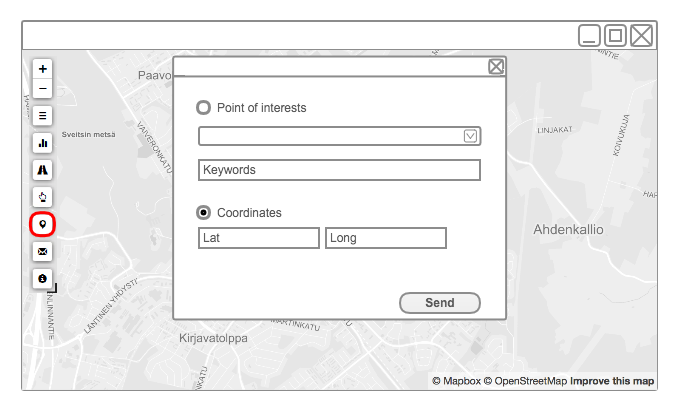
\includegraphics[width=\textwidth]
      {img/c02-application/png/web-basemap-focus.png}
    \caption{Web}
  \end{subfigure}
  ~
  \begin{subfigure}[b]{0.2\textwidth}
    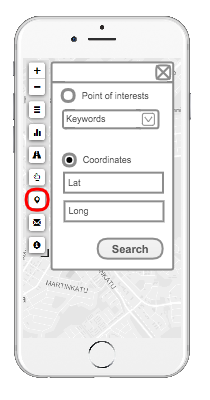
\includegraphics[width=\textwidth]
      {img/c02-application/png/mobile-basemap-focus.png}
    \caption{Mobile}
  \end{subfigure}
  \caption{Application: Focus}
\end{figure}

% CONTACT
% ----------------------------------------------

% FR
Les deux derniers boutons qui doivent être ajoutés ne sont pas nécessaires pour l'application mais simplement utiles et informatifs. Il s'agit des boutons de contact et d'information à propos de l'application. Ces deux boutons ouvre une popup par dessus la carte. Le bouton de contact propose un formulaire permettant de directement envoyer un message aux développeurs de l'application. Quant au bouton d'information, c'est une simple surcouche permettant d'afficher des informations sur les développeurs et les sources de l'application.

% EN
%The last two buttons that need to be added are not necessary for the application but merely useful and informative. These are contact buttons and information about the application. These two buttons open a popup over the map. The contact button provides a form to send a message directly to the developers of the application. As for the information button is a simple overlay that displays information about the developers and the sources of the application.

\begin{figure}[ht]
  \centering
  \begin{subfigure}[b]{0.6\textwidth}
    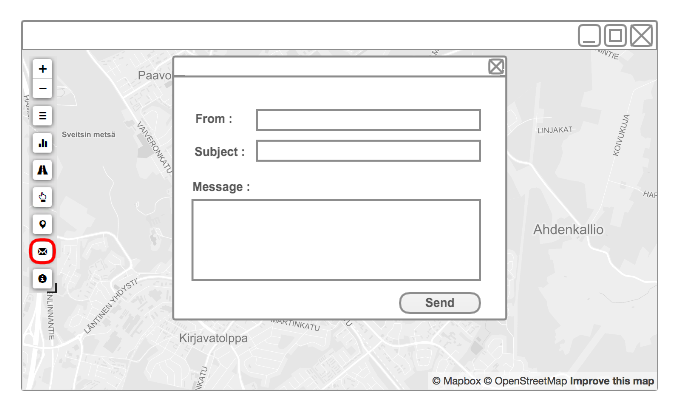
\includegraphics[width=\textwidth]
      {img/c02-application/png/web-basemap-contact.png}
    \caption{Web}
  \end{subfigure}
  ~
  \begin{subfigure}[b]{0.2\textwidth}
    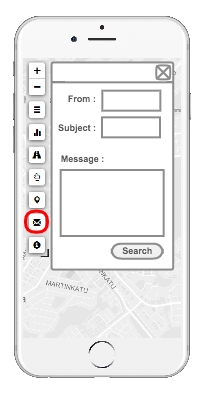
\includegraphics[width=\textwidth]
      {img/c02-application/png/mobile-basemap-contact.png}
    \caption{Mobile}
  \end{subfigure}
  \caption{Application: Contact}
\end{figure}

%%%%%%%%%%%%%%%%%%%%%%%%%%%%%%%%%%%%%%%%%%%%%%%%%%%%%%%%%%%%%%%%%%%%%%%%%

% FR
\subsection{Partie site web}

% EN
%\subsection{Website content}

% FR
Les derniers boutons qui n'ont pas été détaillés dans la partie précédent sont les liens directs vers le mini-site internet. En effet, Il est plus aisé d'aller directement sur le contenu souhaité depuis la carte plutôt que de naviguer sur le site. Parmis les boutons non explicités, on retrouve un bouton d'accès aux statistiques et aux horaires de trains.

% EN
%The last buttons that were not detailed in the previous section are direct links to the Internet website content. Indeed, it is easier to go directly to the desired content from the map rather than browse in the site. Among the non-explicit buttons, we have a button access to statistics and trains timetables.

% STATS
% ----------------------------------------------

% FR
Le site web est composé d'une petite barre de navigation en haut de la page et d'un contenu central. Un lien dans la barre de navigation nous permet de revenir sur la carte. Le contenu central de la page change selon la page désirée. 

Le contenu central de la partie statistique est une liste de schéma et d'un schéma global qui s'actualise selon l'objet sélectionné sur la liste.

% EN
%The website consists of a small top navigation bar and a central content. A link in the navigation bar allows us to go back on the map. The central content of the page changes depending on the desired chart.

%The central content of the statistical part is a charts list and an overall chart that is updated as the selected object on the list.

\begin{figure}[ht]
  \centering
  \begin{subfigure}[b]{0.6\textwidth}
    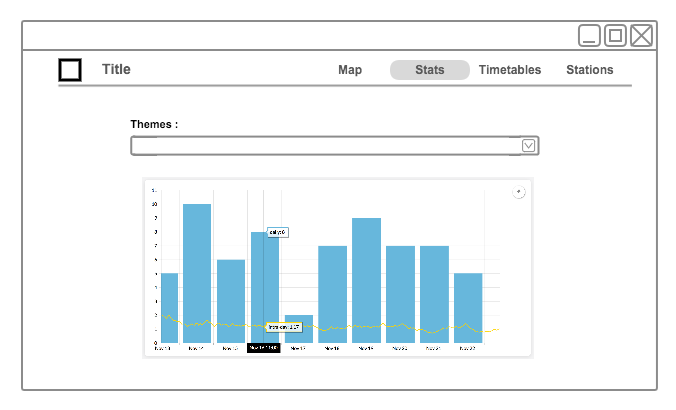
\includegraphics[width=\textwidth]
      {img/c02-application/png/web-website-stats.png}
    \caption{Web}
  \end{subfigure}
  ~
  \begin{subfigure}[b]{0.2\textwidth}
    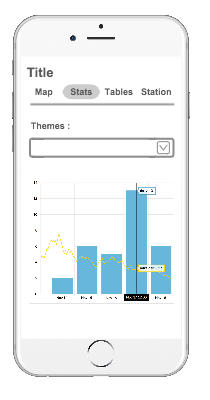
\includegraphics[width=\textwidth]
      {img/c02-application/png/mobile-website-stats.png}
    \caption{Mobile}
  \end{subfigure}
  \caption{Application: Statistics}
\end{figure}

% TIMETABLES
% ----------------------------------------------

% FR
En ce qui concerne les horaires de train, il s'agit d'une interface permettant de récupérer les trains qui intéressent l'utilisateur. L'utilisateur à alors le choix de lister tous les départs de train d'une ville, toutes les arrivées d'une ville ou bien de déterminer l'itinéraire entre deux villes. Une fois le choix fait, l'utilisateur renseigne les villes désirées dans les zones concernées. L'application récupère alors les données et les affiches à l'utilisateur sous forme de liste à ouvrir.

% EN
%Regarding train schedules, it is an interface to retrieve the trains that interest the user. The user then has the choice of listing all train departures of a city, all arrivals to a city or to determine the route between two cities. The choice made, the user fills in the desired towns in the affected areas. The application then retrieves the data and signs the user in a list to open.

\begin{figure}[ht]
  \centering
  \begin{subfigure}[b]{0.6\textwidth}
    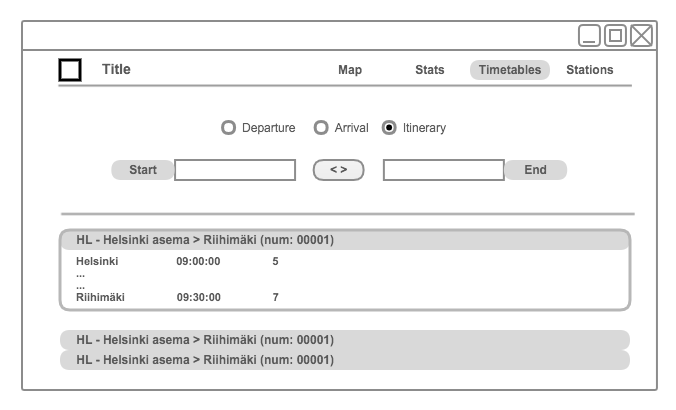
\includegraphics[width=\textwidth]
      {img/c02-application/png/web-website-timetables.png}
    \caption{Web}
  \end{subfigure}
  ~
  \begin{subfigure}[b]{0.2\textwidth}
    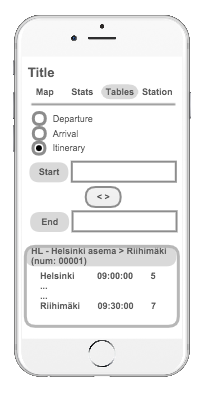
\includegraphics[width=\textwidth]
      {img/c02-application/png/mobile-website-timetables.png}
    \caption{Mobile}
  \end{subfigure}
  \caption{Application: Timetables}
\end{figure}
